\begin{frame}
  \frametitle{Computational Physics Group}
\centerline{\textcolor{blue}{``Complex behavior of disordered systems''}}
\centerline{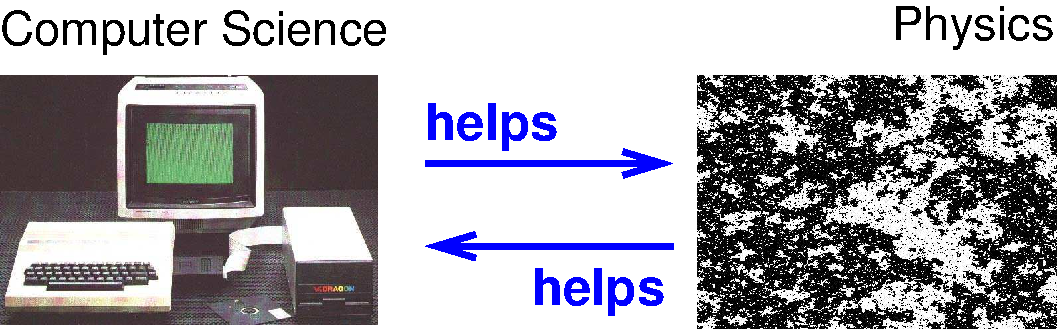
\includegraphics[width=0.6\textwidth]{slide_group/physics_cs}}

\vspace*{2mm}
\begin{minipage}[t]{0.47\textwidth}
{\textcolor{blue}{Computer simulations}}

new algorithms

\begin{center}
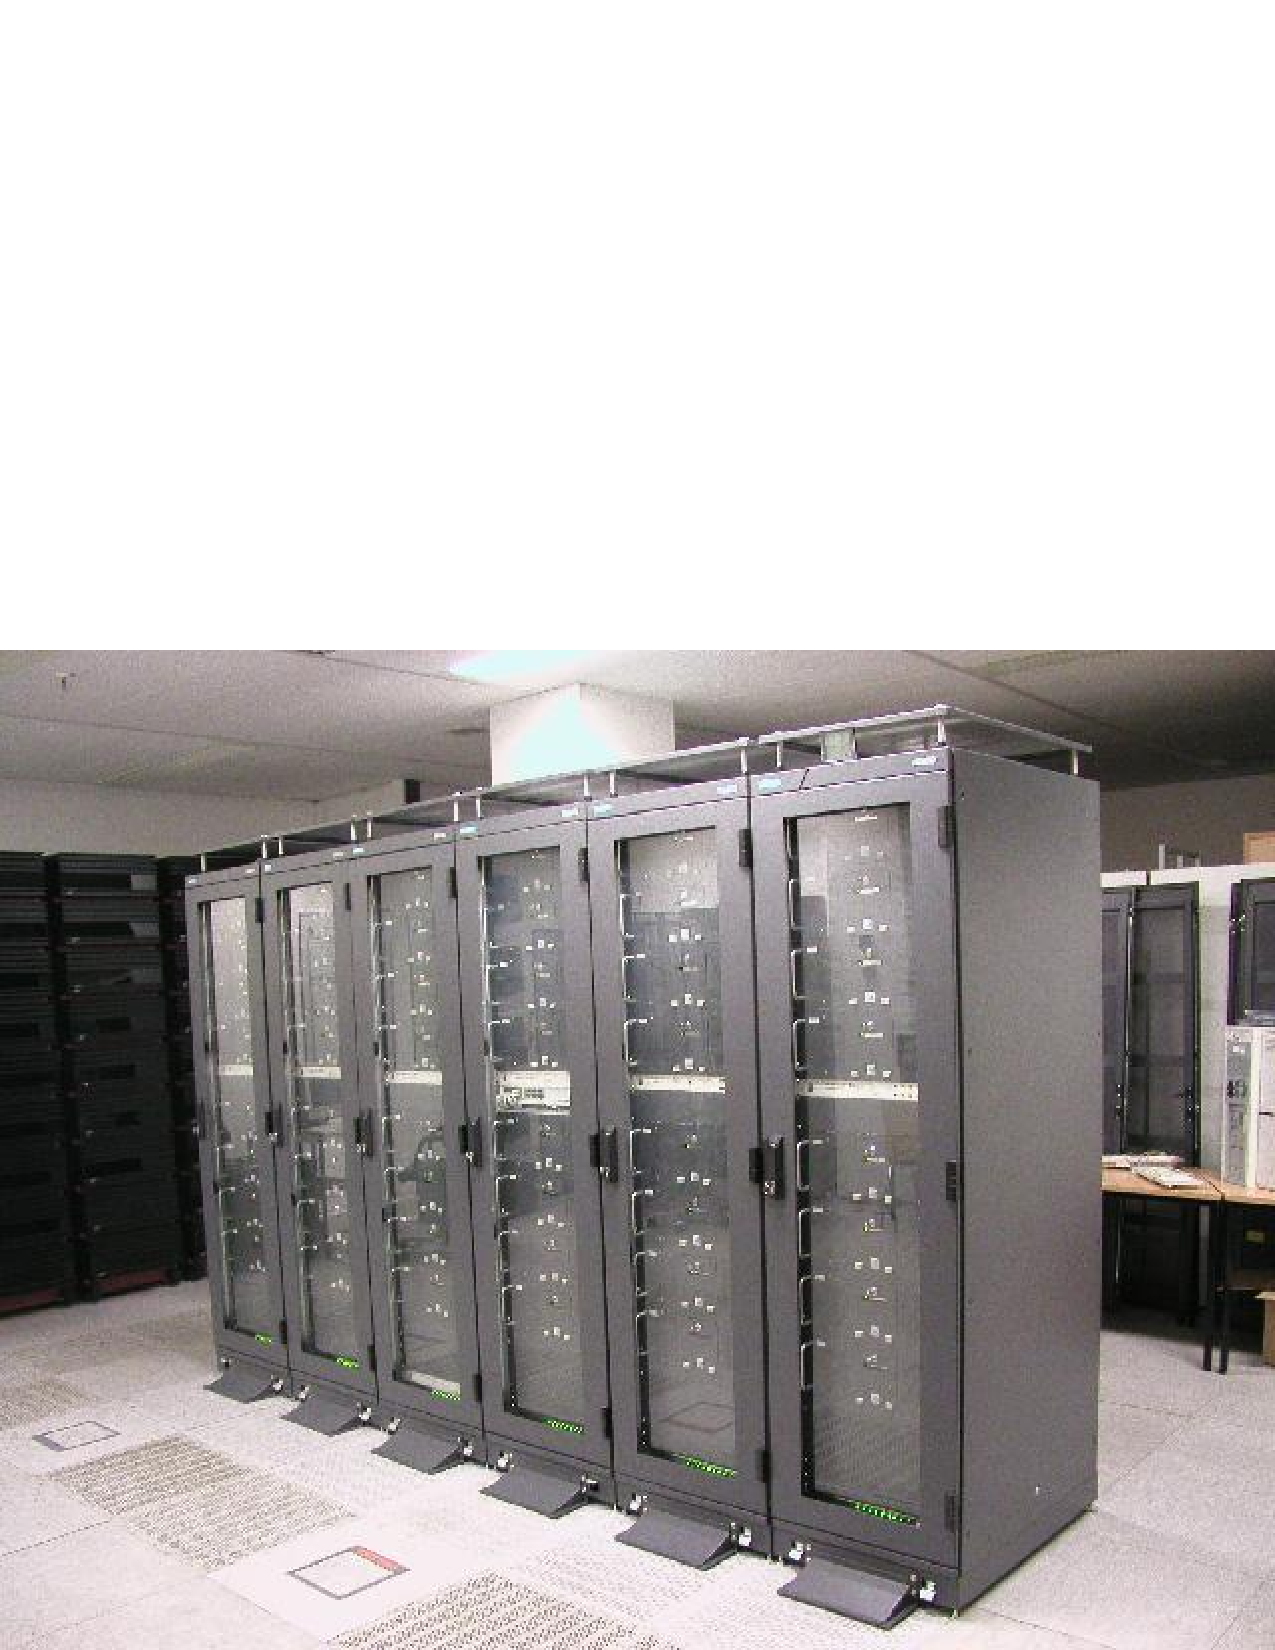
\includegraphics[width=0.6\textwidth]{slide_group/rechner_small}
\rotatebox{90}{
\begin{minipage}[t]{0.4\textwidth}
{\scriptsize [PPCC]}
\end{minipage}
}
\end{center}
\end{minipage}
\hspace*{2mm}
\begin{minipage}[t]{0.47\textwidth}
{\textcolor{blue}{Optimization algorithms}}

development/applications

\begin{overprint}
\onslide<1>\centerline{
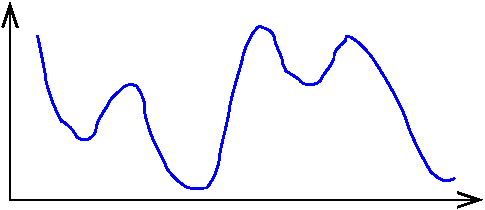
\includegraphics[width=0.8\textwidth,height=0.6\textwidth]
                {slide_group/opt_problem}}
\onslide<2>
\centerline{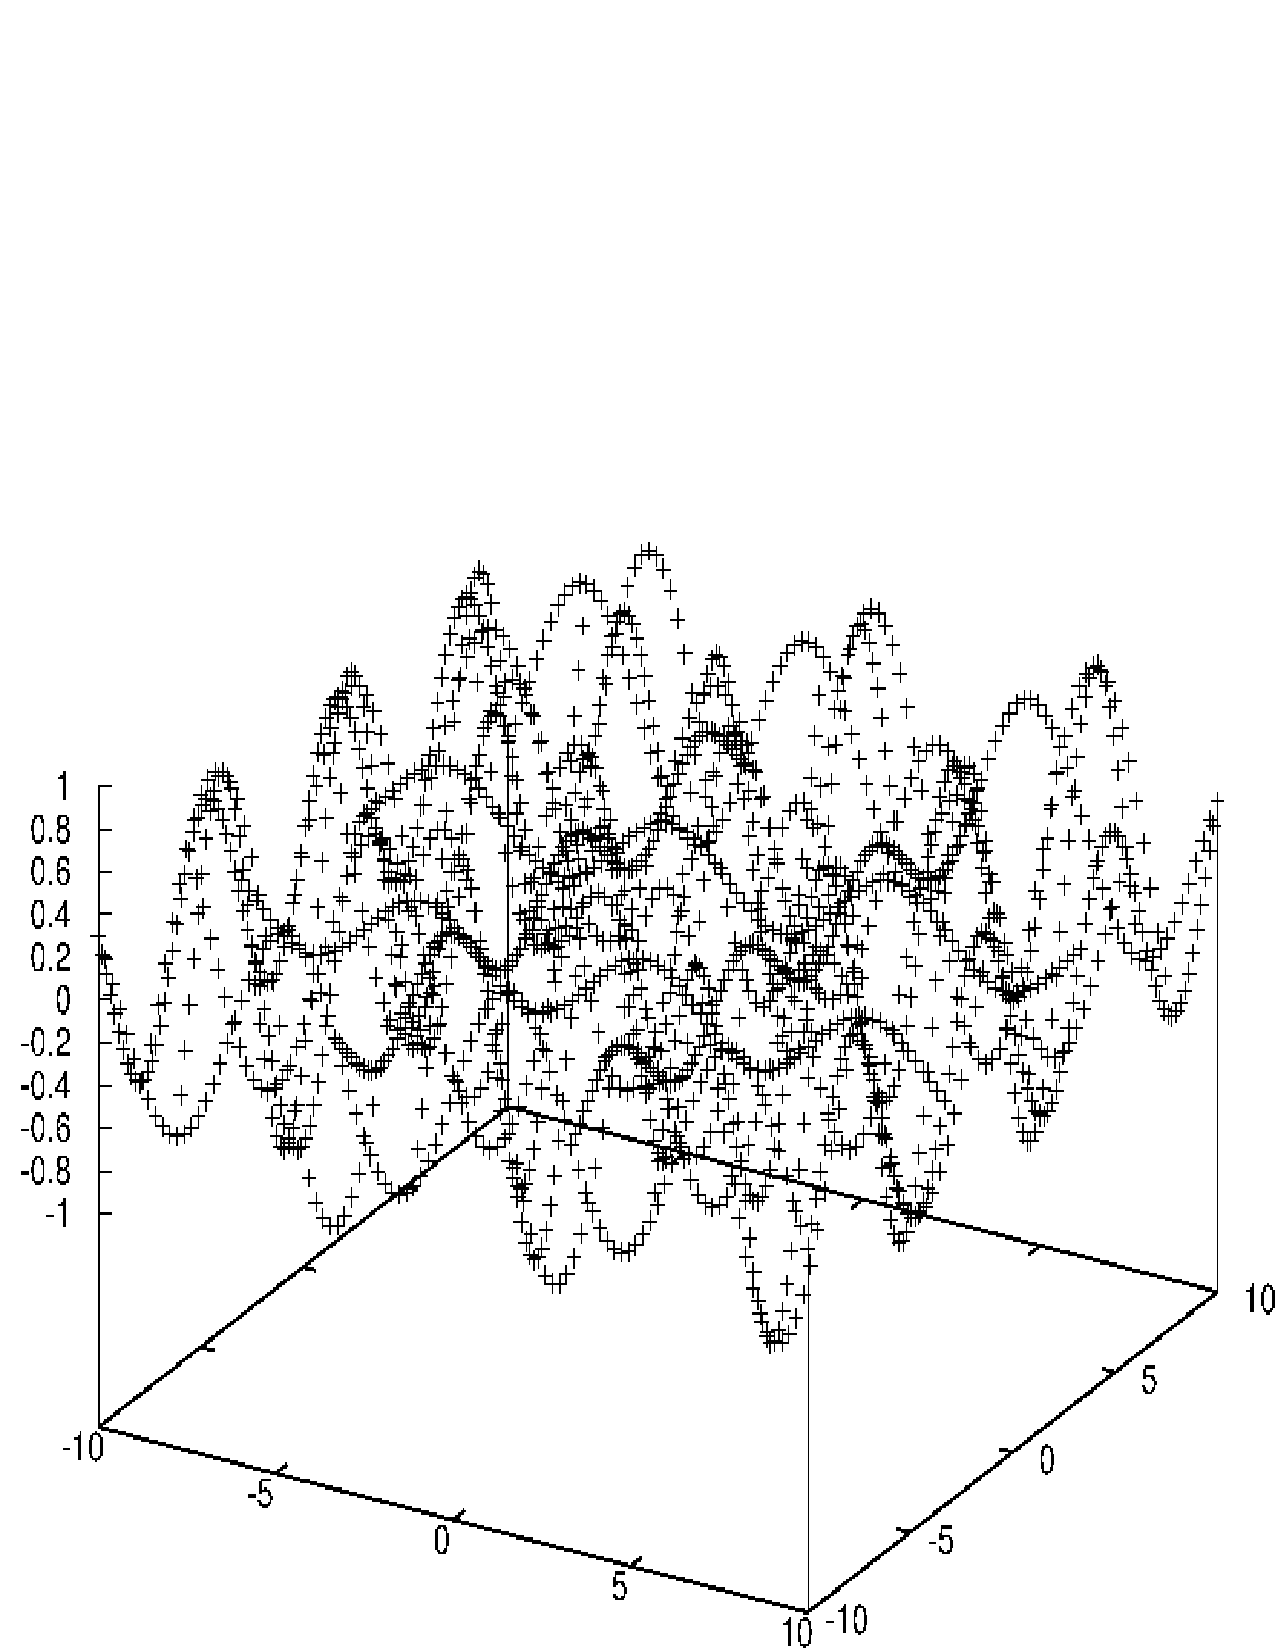
\includegraphics[width=0.9\textwidth,height=0.5\textwidth]
{slide_group/function2dB}}
\end{overprint}
\vspace*{-5mm}
\onslide<2> systems with $10^6$ particles\\[-3mm]
\end{minipage}

{\scriptsize [AKH and H. Rieger, {\it Optimization Algorithms in
    Physics}, Wiley-VCH 2001]}\\[-1.0mm]

\end{frame}

